\begin{minipage}{0.45\linewidth}
		Dans le repère orthonormé \Oijk{}, on considère les points :

		A$(2 ; 1 ; 1)$, B$(3 ;-2 ; 0)$, C$(0 ;-1 ; 1)$ et D$(0 ; 0 ; 2)$.
	\end{minipage}
	\hfill
	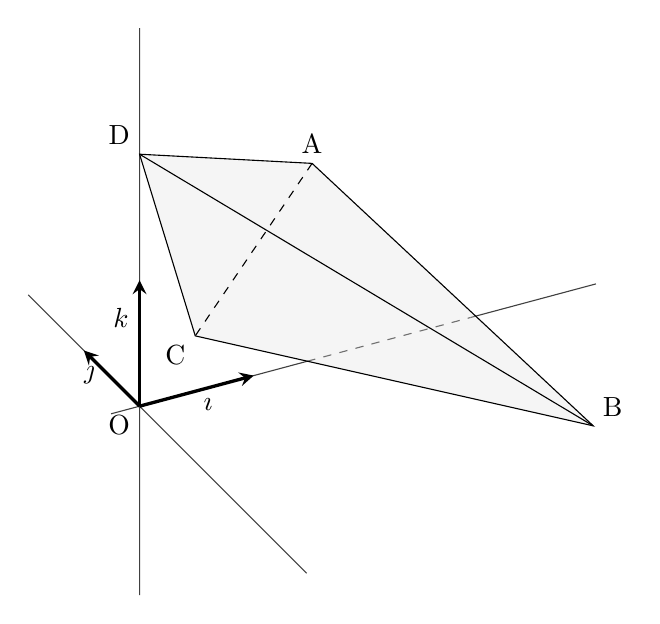
\begin{tikzpicture}[x=(15:15mm),y=(135:10mm),z=(90:16mm),>=stealth,baseline={(current bounding box.center)}]
		\draw[darkgray] (-0.25,0,0)--(1.47,0,0) (2.9,0,0)--(4,0,0)
			(0,-3,0)--(0,2,0)
			(0,0,-1.5)--(0,0,3);
		\draw[darkgray,dashed] (1.47,0,0)--(2.9,0,0) ;
		\draw[->,line width=1.2pt] (0,0,0)--(1,0,0) node[pos=0.6,below]{$\vect{\imath}$} ;
		\draw[->,line width=1.2pt] (0,0,0)--(0,1,0) node[pos=0.9,below]{$\vect{\jmath}$} ;
		\draw[->,line width=1.2pt] (0,0,0)--(0,0,1) node[pos=0.7,left]{$\vect{k}$} ;
		\node at(0,0,0) [below left] {O};
		\foreach \coord/\nom/\pos in {{(2,1,1)}/A/{above},{(3,-2,0)}/B/{above right},{(0,-1,1)}/C/{below left},{(0,0,2)}/D/{above left}}
		{\fill[shift={\coord}] (0,0,0) circle (0.1pt) node[\pos] {\nom} ;}
		\draw[fill opacity=0.3,fill=lightgray!50] (2,1,1)--(3,-2,0)--(0,-1,1)--(0,0,2)--cycle;
		\draw (3,-2,0)--(0,0,2);
		\draw[dashed] (2,1,1)--(0,-1,1) ;
	\end{tikzpicture}


	\begin{enumerate}
		\item Montrer que les points A, B et C définissent un plan.
		\item \begin{enumerate}
			\item Montrer que le vecteur $\vect{n} \begin{pmatrix} 1 \\ -1 \\ 4 \end{pmatrix} $ est normal au plan (ABC).

			\item En déduire qu'une équation cartésienne du plan (ABC) est :
			\[x-y+4 z-5=0.\]
		\end{enumerate}

		\item Vérifier qu'une représentation paramétrique de la droite $\Delta$ passant par D et orthogonale au plan (ABC) est donnée par :
		\[\begin{cases}
			x=t \\
			y=-t \\
			z=2+4 t
		\end{cases} \quad \text { avec } t \in \R.\]
		\item Montrer que le projeté orthogonal de D sur le plan (ABC) est le point H$\left(-\dfrac{1}{6} ; \dfrac{1}{6} ; \dfrac{4}{3}\right)$.
		\item \begin{enumerate}
			\item Montrer que le triangle ABC est isocèle en B.

			\item Montrer que l'aire du triangle ABC est $3 \sqrt{2}$.
		\end{enumerate}

		\item \begin{enumerate}
			\item En déduire que le volume du tétraèdre ABCD est égal à 1.

			\emph{On rappelle que le volume d'un tétraèdre est donné par:} \quad $V=\dfrac{1}{3} \mathcal{B} h$,\quad \emph{ où } $\mathcal{B}$ \emph{est l'aire d'une base et} $h$ \emph{la hauteur relative à cette base.}

			\item On admet que la distance du point A au plan (BCD) est égale à $\sqrt{2}$.

			En déduire l'aire du triangle BCD.
		\end{enumerate}

		\item Dans cette question, on note $\mathrm{D}_{k}$ le point ayant pour coordonnées $(0 ; 0 ; k)$, où $k$ est un réel.
		\begin{enumerate}
			\item Déterminer la valeur de $k$ pour laquelle les points A, B, C et $\mathrm{D}_{k}$ sont coplanaires.

			Quel est alors le projeté orthogonal du point D$_{k}$ sur le plan (ABC)?

			\item Peut-on trouver une valeur de $k$ telle que A soit le projeté orthogonal de $\mathrm{D}_{k}$ sur le plan (ABC) ?
		\end{enumerate}
	\end{enumerate}
